\chapter{Numbers 27}

\begin{figure}
  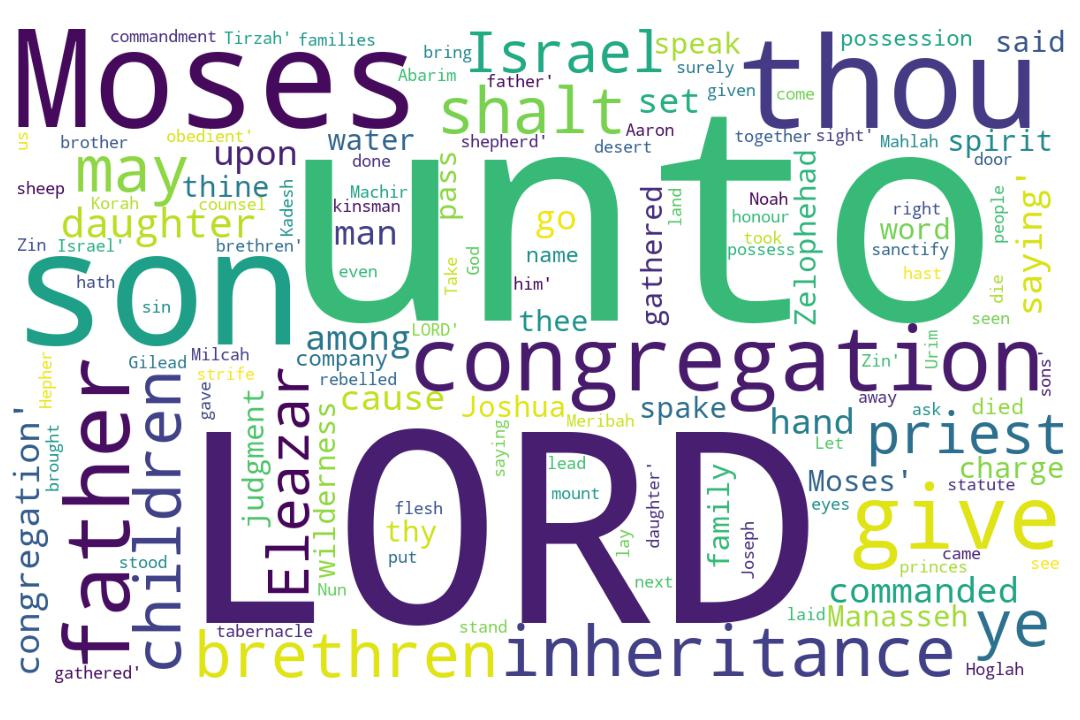
\includegraphics[width=\linewidth]{04OT-Numbers/Numbers27-WordCloud.jpg}
  \caption{Numbers 27 Word Cloud}
  \label{fig:Numbers 27 word Cloud}
\end{figure}

\marginpar{\scriptsize \centering \fcolorbox{blue}{lime}{\textbf{DAUGHTERS OF ZELOPHEHAD}}\\ (Numbers 27)
\begin{compactenum}[I.][8]
    \item \textbf{Single and Dispossessed} \index[scripture]{Numbers!Num 27:01--04} (Numbers 27:2--4)
    \item \textbf{Standing  before the Priests} \index[scripture]{Numbers!Num 27:02} (Numbers 27:2)
    \item A \textbf{Significant Problems} \index[scripture]{Numbers!Num 27:04} (Numbers 27:4)
    \item A \textbf{Sought Possession} \index[scripture]{Numbers!Num 27:04} (Numbers 27:4)
    \item The \textbf{Stated Plan} \index[scripture]{Numbers!Num 27:08--10} (Numbers 27:8--10)
\end{compactenum}}

%%%%%%%%%%%%%%%%%%%%%%%%%%%%%%%%%%
%%%%%%%%%%%%%%%%%%%%%%%%%%%%%%%%%%
\footnote{\textcolor[rgb]{0.00,0.25,0.00}{\hyperlink{TOC}{Return to end of Table of Contents.}}}\footnote{\href{https://audiobible.com/bible/numbers_27.html}{\textcolor[cmyk]{0.99998,1,0,0}{Numbers 27 Audio}}}\textcolor[cmyk]{0.99998,1,0,0}{Then came the daughters of Zelophehad, the son of Hepher, the son of Gilead, the son of Machir, the son of Manasseh, of the families of Manasseh the son of Joseph: and these \emph{are} the names of his daughters; Mahlah, Noah, and Hoglah, and Milcah, and Tirzah.}
[2] \textcolor[cmyk]{0.99998,1,0,0}{And they stood \fcolorbox{bone}{bone}{before} Moses, and \fcolorbox{bone}{bone}{before} Eleazar the priest, and \fcolorbox{bone}{bone}{before} the princes and all the congregation, \emph{by} the door of the tabernacle of the congregation, saying,}
[3] \textcolor[cmyk]{0.99998,1,0,0}{Our father died \fcolorbox{bone}{bone}{in} the wilderness, and he was not \fcolorbox{bone}{bone}{in} the company of them that gathered themselves together against the LORD \fcolorbox{bone}{bone}{in} the company of Korah; but died \fcolorbox{bone}{bone}{in} his own sin, and had no sons.}
[4] \textcolor[cmyk]{0.99998,1,0,0}{Why should the name of our father be done away from among his family, because he hath no son? Give unto us \emph{therefore} a possession among the brethren of our father.}
[5] \textcolor[cmyk]{0.99998,1,0,0}{And Moses brought their cause \fcolorbox{bone}{bone}{before} the LORD.}\\
\\
\P \textcolor[cmyk]{0.99998,1,0,0}{And the LORD spake unto Moses, saying,}
[7] \textcolor[cmyk]{0.99998,1,0,0}{The daughters of Zelophehad speak right: thou shalt surely give them a possession of an inheritance among their father's brethren; and thou shalt cause the inheritance of their father to pass unto them.}
[8] \textcolor[cmyk]{0.99998,1,0,0}{And thou shalt speak unto the children of Israel, saying, If a man die, and have no son, then ye shall cause his inheritance to pass unto his daughter.}
[9] \textcolor[cmyk]{0.99998,1,0,0}{And if he have no daughter, then ye shall give his inheritance unto his brethren.}
[10] \textcolor[cmyk]{0.99998,1,0,0}{And if he have no brethren, then ye shall give his inheritance unto his father's brethren.}
[11] \textcolor[cmyk]{0.99998,1,0,0}{And if his father have no brethren, then ye shall give his inheritance unto his kinsman that is next to him of his family, and he shall possess it: and it shall be unto the children of Israel a statute of judgment, as the LORD commanded Moses.}\\
\\
\P \textcolor[cmyk]{0.99998,1,0,0}{And the LORD said unto Moses, Get thee up into this mount Abarim, and see the land which I have given unto the children of Israel.}
[13] \textcolor[cmyk]{0.99998,1,0,0}{And when thou hast seen it, thou also shalt be gathered unto thy people, as Aaron thy brother was gathered.}
[14] \textcolor[cmyk]{0.99998,1,0,0}{For ye rebelled against my commandment \fcolorbox{bone}{bone}{in} the desert of Zin, \fcolorbox{bone}{bone}{in} the strife of the congregation, to sanctify me at the water \fcolorbox{bone}{bone}{before} their eyes: that \emph{is} the water of Meribah \fcolorbox{bone}{bone}{in} Kadesh \fcolorbox{bone}{bone}{in} the wilderness of Zin.}\\
\\
\P \textcolor[cmyk]{0.99998,1,0,0}{And Moses spake unto the LORD, saying,}
[16] \textcolor[cmyk]{0.99998,1,0,0}{Let the LORD, the God of the spirits of all flesh, set a man over the congregation,}
[17] \textcolor[cmyk]{0.99998,1,0,0}{Which may go out \fcolorbox{bone}{bone}{before} them, and which may go \fcolorbox{bone}{bone}{in} \fcolorbox{bone}{bone}{before} them, and which may lead them out, and which may bring them \fcolorbox{bone}{bone}{in}; that the congregation of the LORD be not as sheep which have no shepherd.}\\
\\
\P \textcolor[cmyk]{0.99998,1,0,0}{And the LORD said unto Moses, Take thee Joshua the son of Nun, a man \fcolorbox{bone}{bone}{in} whom \emph{is} the spirit, and lay thine hand upon him;}
[19] \textcolor[cmyk]{0.99998,1,0,0}{And set him \fcolorbox{bone}{bone}{before} Eleazar the priest, and \fcolorbox{bone}{bone}{before} all the congregation; and give him a charge \fcolorbox{bone}{bone}{in} their sight.}
[20] \textcolor[cmyk]{0.99998,1,0,0}{And thou shalt put \emph{some} of thine honour upon him, that all the congregation of the children of Israel may be obedient.}
[21] \textcolor[cmyk]{0.99998,1,0,0}{And he shall stand \fcolorbox{bone}{bone}{before} Eleazar the priest, who shall ask \emph{counsel} for him after the judgment of Urim \fcolorbox{bone}{bone}{before} the LORD: at his word shall they go out, and at his word they shall come \fcolorbox{bone}{bone}{in}, \emph{both} he, and all the children of Israel with him, even all the congregation.}
[22] \textcolor[cmyk]{0.99998,1,0,0}{And Moses did as the LORD commanded him: and he took Joshua, and set him \fcolorbox{bone}{bone}{before} Eleazar the priest, and \fcolorbox{bone}{bone}{before} all the congregation:}